%% LyX 1.5.5 created this file.  For more info, see http://www.lyx.org/.
%% Do not edit unless you really know what you are doing.
\documentclass[12pt,oneside,english]{amsart}
\usepackage{mathpazo}
\usepackage[T1]{fontenc}
\usepackage[latin1]{inputenc}
\pagestyle{plain}
\usepackage{graphicx}
\usepackage{amssymb}

\makeatletter
%%%%%%%%%%%%%%%%%%%%%%%%%%%%%% Textclass specific LaTeX commands.
\numberwithin{equation}{section} %% Comment out for sequentially-numbered
\numberwithin{figure}{section} %% Comment out for sequentially-numbered
  \@ifundefined{theoremstyle}{\usepackage{amsthm}}{}
  \theoremstyle{plain}
  \newtheorem{thm}{Theorem}[section]

%%%%%%%%%%%%%%%%%%%%%%%%%%%%%% User specified LaTeX commands.
\usepackage{graphicx}

\makeatother

\usepackage{babel}

\begin{document}

\title{Preferences}


\author{Michael Peters}


\date{\today{}}

\maketitle

\section{Introduction}

The foundation of all choice theory in economics is something called
a \textit{preference relation}. The idea is that if I present you
with a pair of alternatives, then you could tell me which one you
prefer, or possibly that you are indifferent between them. The word
'prefer' has different meanings in different contexts. For example,
if I ask you whether you would prefer to see a movie or go to a hockey
game your preference is expressing something about which you would
enjoy. If I ask you whether you would like to have the Olympics in
your local city, your preference may express something about what
you think is best for everyone, or possibly something about what you
think you are supposed to say. Sometimes you really can't say that
one alternative is better than another. For example you might be equally
happy with a ham sandwich or a tuna sandwich. If I allow for that
possibility, it is hard to imagine a situation where you wouldn't
be able to say something.

If I am trying to think about your choice behavior and how I might
understand it, I could begin by trying to imagine all the alternatives
that you could possibly choose. I would collect them together in a
big set $X$. Then I could go about choosing different pairs of alternatives
in $X$ and asking you to express your opinion about which of the
two you prefer. Eventually (as long as you didn't get tired of answering
questions) I could learn which alternative you preferred among any
pair of alternatives in $X$. This collection of information is your
preference relation over $X$.

The set $X$ could be very general. For example, you might have guessed
that we are going to be talking about preference relations over collections
of possible consumption bundles. There is no need to stop there. Much
of modern microeconomic theory arises from thinking about preferences
over things like political parties, environmental policies, business
strategies, location decisions, and so on.

There are many kinds of preference relations you will encounter if
you continue studying economics, but the most widely applied reasoning
in economics assumes that preference relations have two properties
- first, they must be \textit{complete} in the sense that for \textit{any}
pair of alternatives in $X$, either you prefer one or the other,
or are indifferent. There are some interesting preference relations
that are incomplete, but let's leave that for the moment and concentrate
on another problem. Your preference relation could be 'odd'. For example,
suppose you like the Liberals more than the Conservatives because
they are more socially progressive. You might like the NDP more than
the Liberals for the same reason. However, you may prefer the Conservatives
to the NDP because they are more fiscally responsible. Ignoring any
other parties, then you have just expressed a complete and reasonable
preference relation over the political parties. It does present something
of a problem when you are trying to vote. You can't vote Conservative
because you prefer the Liberals to the Conservatives, you can't vote
Liberal because you prefer the NDP to the Liberals. Unfortunately
you can't vote NDP either because you prefer the Conservatives to
the NDP.%
\footnote{I suppose this could explain why so many people don't vote.%
}

We have a word for this kind of preference relation in economics,
it is called an \textit{intransitive} preference relation. To put
this another way, a \textit{transitive} preference relation is one
such that for any 3 alternatives $x$, $y$, and $z$ in $X$, if
$x$ is preferred to $y$ and $y$ is preferred to $z$, then it must
be the case that $x$ is preferred to $z$. A complete transitive
preference relation is called a \textit{rational preference relation}.

In fact, I have just described to you what rationality means in economics.
A person is said to be rational in a particular economic environment
if they have a complete and transitive preference relation over the
alternatives that they face in that environment. In particular, it
doesn't mean that people are greedy or self interested. It doesn't
mean that they are super sophisticated calculators. It just means
that they can express opinions about pairs of alternatives.


\subsection{Behavior}

So how do economists go about predicting what people will do? All
they say is that whatever alternative $x$ is actually chosen from
$X$, then there cannot be another alternative in $X$ that is preferred
to $x$. It is true that in experiments, people sometimes exhibit
intransitive preferences (though they quickly change their behavior
when this is pointed out to them). There are also situations in which
it seems impossible for people to make a choice. For the most part
though, assuming that people are rational (have a complete transitive
preference relation) is pretty innocuous.

It might also occur to you that if you accept that people are rational
decision makers, then you can't really get yourself in too much trouble.
I never said what these preference relations had to look like. To
assert that an individual chooses the alternative that he or she most
prefers is almost tautological. The real content of economic theory
involves restrictions it imposes on $X$ and on the preference relation
over $X$. Its failures and successes having nothing to do with the
assumption of rationality.

Introductory economics courses focus on consumption and consumption
bundles. A consumption bundle is a pair $\left(x,y\right)$ where
the first component of this vector is some quantity that you consume
of one good (just call it good $x$ for short), and the second component
is the quantity you consume of the second good. Consumption doesn't
generate happiness or utility or utils or anything like that. If we
follow your first year course, and imagine that good $x$ has a price
$p$ and good $y$ has a price $q$, and that you have $W$ to spend,
then the consumer faces a set of alternatives $X$ which consists
of all pairs $\left(x,y\right)$ whose cost is less than or equal
to $W$, i.e., \[
X\equiv\left\{ \left(x,y\right)\in\mathbb{R}_{+}^{2}:px+qy\leq W\right\} \]
 Here $\mathbb{R}_{+}^{2}$ is the set of all vectors with two non-negative
components. Read the colon to mean ''such that''.

Well, since we have a set of alternatives, it is pretty safe to assume
that for any pair of alternatives (a pair of alternatives is a pair
of vectors $\left(x,y\right)$ and $\left(x',y'\right)$ here), the
consumer can express a preference between them. Suppose for the moment
that we could get the consumer to tell us what his or her preference
relation is. But now we face a small problem. Suppose the consumer
tells us that he prefers $\left(x,y\right)$ to $\left(x',y'\right)$.
Suppose that we now look at another budget set $X'$ where prices
are $p'$ and $q'$, and maybe income is $W'$. Let's pick this new
set so that it contains both $\left(x,y\right)$ and $\left(x',y'\right)$.
Do we really need to ask the consumer if he prefers $\left(x,y\right)$
to $\left(x',y'\right)$ in this new set? Of course his preference
could well change. People have no use for telephones unless other
people have telephones. The change in income might mean that others
can buy phones. The price changes might signal changes in quality
of the goods that he is buying (suppose $x$ and $y$ are stocks or
bonds or something like that).

Now we begin to impose some restrictions of preferences and economic
theory begins to have some content (of course, we also study what
happens when preference relations change with prices and income).
We are going to assume that if $\left(x,y\right)$ and $\left(x',y'\right)$
are in both $X$ and $X'$ and if $\left(x,y\right)$ is viewed by
the consumer to be at least as good as $\left(x',y'\right)$ in the
preference relation relative to $X$, then it must also be at least
as good as $(x',y')$ in the preference relation relative to $X'$.%
\footnote{This assumption is called the \emph{weak axiom of revealed preference.}%
}

The important point is that the assumption that our consumer was rational
imposed no restriction whatsoever on his behavior. The added assumption
about how his or her preferences are related across different budget
sets does restrict what we should expect to see him do. For example,
suppose that we could run a long series of experiments in which our
consumer is repeatedly asked to choose something from $X$ and that
he consistently chooses $\left(x,y\right)$. If our assumption is
true, then it would be highly unlikely that if we had him choose repeatedly
from $X'$ that he would consistently pick $\left(x',y'\right)$.%
\footnote{He might do this once if he were indifferent, but would probably not
do it consistently if he were indifferent.%
} The predictive content of the theory comes from the assumption that
his preference relation is independent of the prices and income that
he faces, not from the assumption that he is rational.

You will see this repeatedly in economics - we will impose restrictions
on $X$ and the preference relation over it, then make predictions
(and test them). If you want to argue about economics the idea is
to understand these restrictions and criticize them. It is a waste
of time to argue about whether or not consumers are rational.


\subsection{Indifference Curves}

So let's continue with first year economics. Since preference relations
(let's just say preferences from now on) are assumed to be independent
of prices and income, we could sensibly take the consumer's preference
relation and collect together \textit{all} the consumption bundles
$\left(x',y^{\prime}\right)$ which are indifferent to some bundle
$\left(x,y\right)$.%
\footnote{To be formal, we could say that $\left(x,y\right)$ is indifferent
to $\left(x',y'\right)$ if $\left(x,y\right)$ is at least as good
as $\left(x',y'\right)$ and at the same time $\left(x',y'\right)$
is at least as good as $\left(x,y\right)$.%
} As you remember from your first year course, this collection of consumption
bundles is called an \textit{indifference curve}. Please note that
the indifference curve comes directly from the preference relation
and has nothing to do with utils or satisfaction of anything like
that. Since we can construct an indifference curve for any consumption
bundle, there is really a \textit{family} of indifference curves.

Pick two indifference curves in this family, say $C_{1}$ and $C_{2}$
and choose a bundle $\left(x,y\right)$ from $C_{1}$ (which is itself
a set) and $\left(x^{\prime},y'\right)$ from $C_{2}$. If $\left(x,y\right)$
is preferred to $\left(x',y^{\prime}\right)$ then we say that the
indifference curve $C_{1}$ is \textit{higher than} $C_{2}$. Then
of course, any bundle in $C_{1}$ will be preferred to any bundle
in $C_{2}$. There isn't much that can be said about indifference
curves at this point except that when a consumer is rational, two
distinct indifference curves can't have any point in common. To see
this suppose that $C_{1}$ is higher than $C_{2}$. Let $\left(x^{\prime\prime},y^{\prime\prime}\right)$
be the point that the curves have in common, with $\left(x,y\right)$
in $C_{1}$ and $\left(x',y'\right)$ in $C_{2}$. Then $\left(x',y'\right)$
is at least as good as $\left(x^{\prime\prime},y^{\prime\prime}\right)$
since both are in $C_{2}$. $\left(x^{\prime\prime},y^{\prime\prime}\right)$
is at least as good as $\left(x,y\right)$ since both are in $C_{1}$.
Now transitivity requires that $\left(x',y'\right)$ be at least as
good as $\left(x,y\right)$ which is false if the consumer is rational.%
\footnote{A small digression - this simple argument is an example of a line
of reasoning that you will see often in economics. If you want to
show that some property A implies that another property B must be
true, try to show that if $B$ isn't true, then A can't be true either.
This is called a proof \textit{by contradiction.} Here we wanted to
show that if a preference relation is transitive (A) then a pair of
indifference curves couldn't cross (B). We showed that if the curves
did cross, the preference relation couldn't be transitive.%
}

At this point, we could try to describe graphic properties of the
indifference curves. If we started to do that, we would end up spending
considerable time trying to absorb graphic formalism and end up saying
what we could have said with words. So it is time for me to introduce
the theorem that makes economics work.

Write the preference relation as $\succeq$, meaning that $\left(x,y\right)\succeq\left(x',y'\right)$
whenever $\left(x,y\right)$ is preferred to $\left(x',y'\right)$.
A \textit{utility function} is a relation that converts each bundle
$\left(x,y\right)$ into a corresponding utility value or number.
The utility function $u$ represents the preference relation $\succeq$
as long as $u\left(x,y\right)\geq u\left(x',y'\right)$ if and only
if $\left(x,y\right)\succeq\left(x',y'\right)$. If we happened to
be able to find a utility function to represent a preference relation
then we would have a big leg up. To predict what a consumer will do
so far, we need to scan all pairs of consumption bundles until we
find a bundle such that no other bundle is preferred to it. This makes
for a lot of tedious pairwise comparisons. There isn't any obvious
reason why this sort of reasoning is going to help us understand behavior.
If preferences are represented by a utility function, we could take
the function and find the bundle that produced the highest utility
number in the set of alternatives. That would be relatively easy because
we could use all the standard mathematical tricks we know about maximizing
functions (like setting derivatives to zero and so on).

Yet the utility function yields something far more important. As I
mentioned above, the content of economic theory doesn't come from
the rationality assumption. It comes from imposing restrictions on
the preference relation and the feasible set. It is difficult to formulate
ideas about preference relations since they are relative complex objects.
On the other hand, it is much easier to impose and understand restrictions
on utility functions.

Assuming that people have utility functions which they maximize is
just about the last thing we want to do. If we did that, then all
the people who accuse economists of being irrelevant because they
assume that consumers are 'rational' would have a good point. We would
be guilty of predicting behavior by assuming that people do something
that they obviously don't.

So why use a utility function? We need to add one important restriction
on preference relations, and one simplifying restriction.%
\footnote{Simplifying means that I could make the same argument I am about to
make without the restriction, but it would take me a lot longer.%
} The simplifying restriction is that our consumer likes more of both
goods - i.e., if $\left(x,y\right)$ and $\left(x',y'\right)$ are
such that $x\geq x^{\prime}$ and $y\geq y'$ then $\left(x,y\right)\succeq\left(x',y'\right)$.
Furthermore, if one of the inequalities is strict, we will assume
that it is not true that $\left(x^{\prime},y^{\prime}\right)\succeq\left(x,y\right)$.
Having more of any good makes the consumer strictly better off. For
short, let's say that such a preference relation is \textit{monotonic}.

Now for the important restriction. The set of bundles that are at
least as good as $(x,y)$ is given by $B=\left\{ \left(x^{\prime},y^{\prime}\right)\in\mathbb{R}_{+}^{2}:\left(x^{\prime},y^{\prime}\right)\succeq\left(x,y\right)\right\} $.
The set of consumption bundles that are no better than $(x,y)$ is
given by $W=\left\{ \left(x',y'\right)\in\mathbb{R}_{+}^{2}:\left(x,y\right)\succeq\left(x',y'\right)\right\} $.
The important assumption is that both $B$ and $W$ are \textit{closed}
sets%
\footnote{A closed set is one for which any convergent sequence of points in
the set converges to a point in the set. The set $\{x:0\leq x\leq1\}$is
closed, the set $\{x:0<x<1\}$ is open. The complement of a closed
set is open, and conversely. Some sets are neither open nor closed,
for example $\{x:0<x\leq1\}$.%
}. If the sets $B$ and $W$ are both closed for any $\left(x,y\right)\in\mathbb{R}_{+}^{2}$
then the preference relation is said to be \textit{continuous.} Now
the following important theorem is true:

\begin{thm}
Let $\succeq$ be a continuous and monotonic rational preference relation.
Then there exists a utility function $u$ which represents the preference
relation $\succeq$. 
\end{thm}
\begin{proof}
We are going to prove this constructively by actually making up the
function. This function converts every point in $\mathbb{R}^{2}$
into a point in $\mathbb{R}$. 

First some preliminaries. Let $Z$ represent the 45$^{0}$ line (i.e.,
the set of all points in $\mathbb{R}_{+}^{2}$ which have the same
horizontal and vertical coordinate). Let $\left(x,y\right)$ be any
consumption bundle. The bundle $\left(\max\left[x,y\right],\max\left[x,y\right]\right)$
is in $Z$ and is at least as good as $\left(x,y\right)$ by the fact
that preferences are monotonic. Similarly $\left(x,y\right)$ is preferred
to $\left(\min\left[x,y\right],\min\left[x,y\right]\right)$ by monotonicity.
So the sets $P^{+}\equiv B\cap Z$ and $P^{-}\equiv W\cap Z$ are
both non-empty. As preferences are continuous, these sets are both
closed. This lets us deduce that the sets $P^{+}$ and $P^{-}$ are
both closed as they are both intersections of closed sets. 

In Figure \ref{g1} the set $P^{+}$ is marked in red. It is the intersection
of the 45$^{0}$ line and the set $B$ consisting of all bundles that
are preferred to $\left(x,y\right)$. The set $P^{-}$ is marked in
blue in the figure.

Now the sets $P^{+}$ and $P^{-}$ are made up of bundles (in $\mathbb{R}_{+}^{2}$)
that have the same horizontal and vertical component. So, we can associate
each bundle in $Z$ with this common component, which is just a positive
real number. Since each bundle $z\in Z$ either has $z\succeq\left(x,y\right)$
or $\left(x,y\right)\succeq z$ by the completeness of preferences,
(recall that completeness is part of rationality) each point in $Z$
is either in $P^{+}$ or $P^{-}$. Each point in $P^{+}$ or $P^{-}$
is also in $Z$ by construction, so $Z=P^{+}\cup P^{-}$.

We will now demonstrate that the sets $P^{+}$ and $P^{-}$ share
exactly one point in common. Part of the argument for this is an arcane
point in set theory. Since $P^{+}\cup P^{-}$ is all of $Z$, if they
don't share a common point, then $P^{-}$ must be the complement of
$P^{+}$ in $Z$. Since the complement of a closed set is open, $P^{-}$
would have to be open which we have already argued cannot be the case.
So there must be at least one common point. Could there be two? Again,
suppose there were, say $z$ and $z'$. They are both in $Z$ so they
are both on the 45$^{0}$ line. If they are distinct then, say, $z>>z'$
(meaning each component of $z$ is strictly larger than the corresponding
component of $z'$). Then by monotonicity $z\succeq z'$ but not the
other way around. Lets just say that $z\succ z^{\prime}$ so we don't
have to add {}``not the other way around'' all the time. Since $z\in P^{-}=Z\cap W$,
$\left(x,y\right)\succeq z$. Since $z\succ z^{\prime}$, we must
have $\left(x,y\right)\succ z'$ since preferences are transitive.
But this is inconsistent with $z'\in P^{+}$.

All this work leads to the conclusion that for every bundle $\left(x,y\right)$
we can find a point on the 45$^{0}$ line which is indifferent to
it. Let's simply call the common coordinate of this point the \textit{utility}
$u\left(x,y\right)$ associated with the bundle $\left(x,y\right)$
(this emphasizes the point that utility is measured as some number
of goods, not as utils or satisfaction).

Finally, all we need to do is check that this utility function $u\left(x,y\right)$
actually represents preferences. This is pretty straightforward. For
example if $u\left(x,y\right)\geq u\left(x',y^{\prime}\right)$ then
the $z$ associated with $\left(x,y\right)$ has a bigger common component
than the $z'$ associated with $\left(x^{\prime},y'\right)$. Then
$\left(x,y\right)\succeq z$ (since $z\in P^{-}$ for $\left(x,y\right)$)
$\succeq z'$ (by monotonicity) $\succeq\left(x',y'\right)$ (since
$z'\in P^{+}$ for $\left(x',y'\right)$). The other direction is
just as easy. 
\end{proof}
%
\begin{figure}
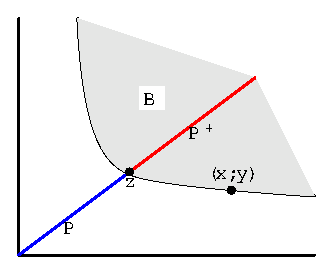
\includegraphics{preferences_fig1}

\caption{\label{g1}The sets $P^{+}$ and $P^{-}$}

\end{figure}


So let's collect our thoughts for a moment. When a consumer chooses
a bundle from some budget set, she picks something such that if we
offer her some other bundle from the same budget set, she will not
want it. If her preferences are transitive and complete (and continuous)
it will \textit{appear to be the case} that she is choosing a bundle
to maximize a utility function subject to the budget constraint. In
the consumer's own mind, there is no such thing as utility: rational
utility maximization is an implication of simpler properties of consumer
behavior. Nor is it assumed that there is any numerical way to measure
happiness or satisfaction. These simply aren't parts of modern microeconomic
theory.


\subsection{Economic Modeling}

Why was this theorem so important? Well it shows first that economic
methodology itself doesn't rely on grand assumptions about human behavior.
Of course, when we impose restrictions on the preference relation
or the set of feasible alternatives, we are making assumptions. These
assumptions are part of what we call economic \textit{models}. When
we formulate an economic model, we try to extract all the implications
of the restrictions. These restrictions are predictions the model
makes. We can collect data about the choices consumers actually do
make, to check whether these predictions are right. When they are
wrong, we know we need to reformulate the model (or change some of
the restrictions).

The second thing is shows is that we can extract these restrictions
using some fairly basic mathematical tools, like the theory of optimization
(and of course, the dreaded calculus). The mathematization of economics
occurred in the late 50's and has had a remarkable impact on the way
economists interact. To use mathematics, it is necessary that the
concepts, sets, and functions involved be very precisely defined.
There is no room for interpretation (though certainly there is room
to fine tune and modify concepts). An economic concept must mean the
same thing to everyone.

This has had an impact that you might not expect. Anyone who understands
basic mathematics should be able to understand the most advanced ideas
in economic theory. Oddly enough mathematics makes economics very
inclusive.%
\footnote{You might like to compare the definition of utility I have given above
with definitions you will hear for important concepts like capitalism
or post modernism.%
} This has had great benefits for economist, since other fields have
been moving in much the same direction. Computer science, biology,
ecology, environmental science, all use methods similar to those used
by economists. The level of interaction among practitioners in these
different fields is increasing to the enrichment of all.

Most of this course tries to develop the mathematical and conceptual
tools you need to formulate and analyze economic models on your own.
As we go about this, you will see some models that have worked out
pretty well in the sense that they give very good insight into some
pretty applied problems. You will also get a chance to see some models
that don't work so well. These 'failures' give a good deal of insight
into how theoretical and empirical work interact. Though these applications
are important in the overall scheme of things, they are not the main
focus of the course. It is the art of building the models themselves
that is the concern here. Once you begin to appreciate this approach,
your subsequent studies in more applied areas will make more sense.


\subsection{Addendum: Are People Rational in the sense that Economists use the
term?}

Since people always make choices, it is pretty find a violation of
the assumption that 'preferences' are complete. It is possible to
'test' transitivity. This test will be discussed later. However, the
implications of rationality are always part of a joint hypothesis.
For example, in the standard consumer model, predictions come from
the assumption that people are rational \textbf{and} from the assumption
that their preferences don't change when you present them with different
budget constraints. The classical theory of demand and markets that
is taught in first year economics courses comes more from assumptions
that are tacked on in addition to rationality.

I'll mention a few famous arguments. One example, due to Tversky and
Kahneman (1981) refers to something that is now referred to as a 'framing
effect'. Subjects are presented with a hypothetical situation in which
they need to make a medical decision in response to a new disease.
There are 600 people who have been exposed to a new and lethal virus.
One of two vaccines can be produced. The first will save 200 of them
for sure. The other has a $\frac{1}{3}$ chance of saving all 600,
but a $\frac{2}{3}$ chance of being completely ineffective. Call
the first vaccine $a$, and the second vaccine $b$. Some people choose
$a$ some choose $b$ (there is no answer here, it is just a choice).
In the second experiment, the same subjects are offered a choice between
the following two vaccines. Adopting vaccine $c$ will result in 400
people dying for sure. With vaccine $d$ there is a $\frac{2}{3}$
chance that all 600 will die, but a $\frac{1}{3}$ chance that none
of them will die. In their experiments, most people who chose vaccine
$a$ over vaccine $b$ proceeded to choose vaccine $d$ over vaccine
$c$.

If you think about it for a moment, you should see that in terms of
physical outcomes, vaccines $a$ and $c$ are identical, while vaccines
$b$ and $d$ are identical. In terms of consumer theory, people who
were offered the same hypothetical budget made different choices in
the two situations. One of the most basic assumptions of consumer
theory seems to have been violated. Of course, since no evidence of
intransitivity is presented, this isn't a contradiction of rationality.%
\footnote{It might have occurred to you that asking people what they would do
in a hypothetical situation is not likely to elicit much useful information.
People are more likely to tell you what they think you want to hear,
than what they actually prefer. The experiment was also run with the
vaccine story replaced by monetary bets - similar results applied. %
}

Another famous example, again due originally to Khaneman and Tversky,
has to do with something called an \emph{anchoring} effect. The choice
experiment was carried out by Ariely Lowenstein and Prelec (maybe
2003). MBA students were asked whether they were willing to buy consumer
items (computer keyboards, wireless mice, wine, chocolates, etc) for
a dollar price which was equal to the last two digits of their social
security number. This is the same as asking whether you would be willing
to pay a price equal to the last two digits of of your student number.
If the last two digits were 25, then the computer keyboard was yours
for \$25 (US of course). Their answer was simply recorded. No transaction
actually occurred at this point. Then the actual price they were willing
to pay was elicited in a manner that made them report the price truthfully.%
\footnote{I am not sure exactly what method was used, but one way to do this
is as follows: you ask the student for a price between $0$\$ and
$100\$$, and then draw a price randomly in the same range using a
computer. If the price named by the student is higher, then the student
can buy the article and pays the price that was chosen by the computer.
If the computer's price is higher, then there is no transaction. I
leave it to you to see if you can figure out why the student should
name a price that is equal to their true willingness to pay.%
}

The interesting result - a strong correlation between the last two
digits of the students id, and their willingness to pay. In one example,
students whose last two digits were below 50 ended up, on average
willing to pay 11\$ for a bottle of wine, while students whose last
two digits were above 50 wanted to pay almost \$20 for the same wine.
I suppose it is possible that numbers have karma, and people with
large digits at the end of their social security numbers end up being
richer (and so can afford to pay more for wine). More mundanely, a
preference ordering over money and wine seems to depend on things
that appear irrelevant. 

I point these things out for two reasons. First, to illustrate that
rationality itself is not typically at the root of the problem in
these studies, it is much stronger assumptions about the nature of
preferences that these studies call into question. We will come upon
other examples like this as we go along.

Second, I want to point out that, though we won't get to much of it
in this course, economic theory has presented models to deal with
these kinds of behavior, all based on exactly the assumption of complete
and transitive preferences that we will use here. Most important,
economic theory has recognized that almost all decisions are made
with very limited information. The examples above are a bit like that.
How to weigh the value of 400 lives in the first example against 600
uncertain lives; what exactly does it mean $\frac{1}{3}$ probability.
In these kind of situations people make choices even though they don't
really understand what the choices involve. We touch on this issue
later when we discuss the expected utility theorem.

One of the most important kinds of problems that economists study
are those in which the best action for me depends on what other people
do. I don't want to buy a theatre ticket unless my friend wants to
go to the theatre with me. The motivations of others are perhaps the
most uncertain thing of all. This is the purview of game theory, which
we will again be forced to visit briefly when we discuss externalities
below.

It is the methods and art of economic modelling that the material
in this course is meant to illustrate. It is exactly these methods
that will later make it possible to understand situations that are
more complex than those discussed in consumer theory.
\end{document}
